
%\RequirePackage{pdf15}

\documentclass{beamer}

\usepackage[utf8]{inputenc}

\usepackage{mystyle}
\usepackage{algorithm}
\usepackage[noend]{algorithmic}

\usepackage{tikz}
\usepackage{pgfplots}
\usepackage{subcaption}

%\usepackage{natbib}
\usepackage[style=authortitle,backend=biber]{biblatex}
\addbibresource{anthology.bib}
\addbibresource{emnlp2020.bib}
\renewcommand{\footnotesize}{\scriptsize}

\usepackage{tikz-dependency}
\usetikzlibrary{shapes.arrows, positioning, fit, bayesnet,
    arrows,backgrounds,patterns,matrix,calc,shadows,plotmarks,
    shapes,positioning,automata,positioning,spy,scopes,chains,decorations,decorations.pathreplacing}

\newcommand{\FancyUpArrow}{
\begin{tikzpicture}[baseline=-0.3em]
\node[single arrow,draw,rotate=90,single arrow head extend=0.2em,inner
ysep=0.2em,transform shape,line width=0.05em,top color=green,bottom color=green!50!black] (X){};
\end{tikzpicture}}
\newcommand{\FancyDownArrow}{
\begin{tikzpicture}[baseline=-0.3em]
\node[single arrow,draw,rotate=-90,single arrow head extend=0.2em,inner
ysep=0.2em,transform shape,line width=0.05em,top color=red,bottom color=red!50!black] (X){};
\end{tikzpicture}}

\AtBeginSection[]{
  \begin{frame}
  \vfill
  \centering
  \begin{beamercolorbox}[sep=8pt,center,shadow=true,rounded=true]{title}
    \usebeamerfont{title}\insertsectionhead\par%
  \end{beamercolorbox}
  \vfill
  \end{frame}
}

% quotes
\usepackage[style=british]{csquotes}

\def\signed #1{{\leavevmode\unskip\nobreak\hfil\penalty50\hskip1em
  \hbox{}\nobreak\hfill #1%
  \parfillskip=0pt \finalhyphendemerits=0 \endgraf}}

\newsavebox\mybox
\newenvironment{aquote}[1]
  {\savebox\mybox{#1}\begin{quote}\openautoquote\hspace*{-.7ex}}
  {\unskip\closeautoquote\vspace*{1mm}\signed{\usebox\mybox}\end{quote}}

%Information to be included in the title page:
\title{Low-Rank Factorizations for Fast Inference in Structured Models}
\author{Justin Chiu* \inst{1} \and Yuntian Deng* \inst{2} \and Alexander Rush \inst{1}}
\institute[shortinst]{\inst{1} Cornell Tech \and \inst{2} Harvard University}

\setbeamertemplate{navigation symbols}{} 
\setbeamertemplate{footline}[frame number]

% hypergraph

 
\begin{document}

\begin{frame}[plain]
\titlepage
\end{frame}

\begin{frame}
\frametitle{Structured Models}
\begin{itemize}
\item Explicitly model output associations
    \begin{itemize}
    \item Directly or through latent variables
    \end{itemize}
\vspace{1em}
\item Focus on combinatorially large latent \underline{discrete structures}
    \begin{itemize}
    \item Complementary to continuous, deterministic representations
    \end{itemize}
\vspace{1em}
\item More difficult to scale than alternative representations
\begin{itemize}
    \item Bottlenecked by time + space complexity of marginal inference
    \end{itemize}
\end{itemize}
\end{frame}

\begin{frame}
\frametitle{Scaling Structured Models}

\begin{itemize}
\item Scaling (to the point of overparameterization) is key
\vspace{1em}
\item Target tractable models
    \begin{itemize}
    \item Admit dynamic programs for exact marginalization
    \end{itemize}
\vspace{1em}
\item Impose a low-rank model constraint
    \begin{itemize}
    \item Trades off model expressivity for cheaper marginalization
    \end{itemize}
\vspace{1em}
\item Only constrain parameters used in key steps of marginalization
\end{itemize}
\end{frame}

\begin{frame}
\frametitle{Marginalization in Structured Models}
\begin{itemize}
\item Model an observation $x = (x_1,\ldots,x_T)$ via latent structure $z$
    \begin{itemize}
    \item Latent nodes $z_i$
    \item Nodes have discrete label set $[L]$
    \end{itemize}
\vspace{1em}
\item Perform training and evaluation via marginalization
    $$p(x) = \sum_z p(x,z)$$

%\item Two examples:

\begin{columns}

\begin{column}{0.5\textwidth}
\begin{center}
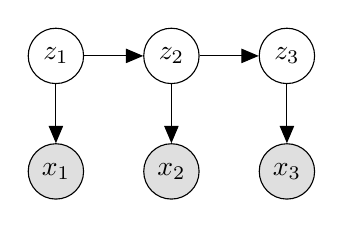
\begin{tikzpicture}[]
\node[latent] (z0) {$z_1$} ;
\node[latent] (z1) [right=0.75cm of z0] {$z_2$} ;
\node[latent] (z2) [right=0.75cm of z1] {$z_3$} ;

\node[obs]    (x0) [below = 0.75cm of z0] {$x_1$};
\node[obs]    (x1) [below = 0.75cm of z1] {$x_2$};
\node[obs]    (x2) [below = 0.75cm of z2] {$x_3$};

\edge {z0} {x0};
\edge {z1} {x1};
\edge {z2} {x2};
\edge {z0} {z1};
\edge {z1} {z2};
\end{tikzpicture}

\vspace{1.1em}
\small{Hidden Markov models}
\end{center}
\end{column}

\begin{column}{0.5\textwidth}
\begin{center}
\begin{tikzpicture}
\node[const, inner sep=.4em] (z0) {$z_1$} ;
\node[const, inner sep=.4em] (z1) [below left=0.5cm and 0.5cm of z0] {$z_2$} ;
\node[const, inner sep=.4em] (z2) [below right=0.5cm and 0.5cm of z0] {$z_3$} ;

%\node[obs]    (x0) [below left = 0.5cm and 0.1cm of z1] {$x_1$};
%\node[obs]    (x1) [below right = 0.5cm and 0.1cm of z1] {$x_2$};
%\node[obs]    (x2) [below left = 0.5cm and 0.1cm of z2] {$x_3$};
%\node[obs]    (x3) [below right = 0.5cm and 0.1cm of z2] {$x_4$};
\node[const, inner sep=.4em]    (x0) [below left = 0.5cm and 0.1cm of z1] {$x_1$};
\node[const, inner sep=.4em]    (x1) [below right = 0.5cm and 0.1cm of z1] {$x_2$};
%\node[const, inner sep=.4em]    (x2) [below left = 0.5cm and 0.1cm of z2] {$x_3$};
%\node[const, inner sep=.4em]    (x3) [below right = 0.5cm and 0.1cm of z2] {$x_4$};
\node[const, inner sep=.4em]    (x2) [below = 0.5cm of z2] {$x_3$};

\edge[-] {z0} {z1};
\edge[-] {z0} {z2};
\edge[-] {z1} {x0};
\edge[-] {z1} {x1};
\edge[-] {z2} {x2};
%\edge[-] {z2} {x3};
\end{tikzpicture}

\vspace{.11em}
\small{Probabilistic context-free grammars}
\end{center}
\end{column}

\end{columns}
\end{itemize}

\end{frame}

\begin{frame}
\frametitle{Hypergraphs for Marginalization}
\begin{itemize}
\item Represent marginalization dynamic programs as hypergraphs
\vspace{1em}
\item Hypergraphs consist of nodes and hyperedges
    \begin{itemize}
    \item Hyperedge consists of a head node and set of tail nodes
    \end{itemize}
\vspace{1em}
\item Perform marginalization by traversing hypergraph
    \begin{itemize}
    \item Aggregate marginals from tails to head via a matrix-vector product
    \end{itemize}
\end{itemize}
\begin{columns}

\begin{column}{0.5\textwidth}
\begin{center}
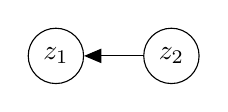
\begin{tikzpicture}[]
\node[latent] (z0) {$z_1$} ;
\node[latent] (z1) [right=.75cm of z0] {$z_2$} ;

\edge {z1} {z0};
\end{tikzpicture}
\end{center}
\end{column}

\begin{column}{0.5\textwidth}
\begin{center}
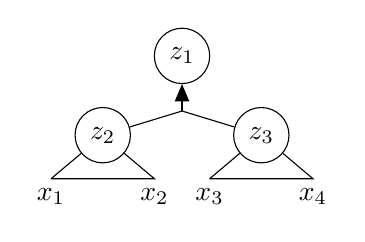
\begin{tikzpicture}
%\node (a) [minimum height = 1.5em] {$x_1$};
%\node (b) [right=of a, minimum height = 1.5em] {$x_2$};
%\node (b2) [right=.2em of b, minimum height = 1.5em] {$x_3$};
%\node (c) [right=of b2, minimum height = 1.5em] {$x_4$};
%\coordinate (bbx) at ($ (b.north) + (b2.north) $);

%\coordinate (abx) at ($ (a.north) + (b.north) $);
%\coordinate [label=above left:{B}] (ab) at ($ 0.5*(abx) + (0,1) $);
%\draw (a.north) -- (b.north) -- (ab) -- cycle;
%\coordinate (bcx) at ($ (b2.north) + (c.north) $);
%\coordinate [label=above right:{C}] (bc) at ($ 0.5*(bcx) + (0,1) $);
%\draw (b2.north) -- (c.north) -- (bc) -- cycle;

%\coordinate (abc) at ($ 0.5*(bbx) + (0,1.5) $);
%\node (d) at ($ 0.5*(bbx) + (0,2.5) $) {A};

%\draw (ab) -- (abc);
%\draw (bc) -- (abc);
%\draw [->] (abc) -- (d);

\node[latent] (z0) {$z_1$} ;
\node[latent] (z1) [below left=0.5cm and 0.5cm of z0] {$z_2$} ;
\node[latent] (z2) [below right=0.5cm and 0.5cm of z0] {$z_3$} ;

\node    (x0) [below left = 0.3cm and 0.1cm of z1] {$x_1$};
\node    (x1) [below right = 0.3cm and 0.1cm of z1] {$x_2$};
\node    (x2) [below left = 0.3cm and 0.1cm of z2] {$x_3$};
\node    (x3) [below right = 0.3cm and 0.1cm of z2] {$x_4$};

\draw (x0.north) -- (x1.north) -- (z1) -- (x0.north);
\draw (x2.north) -- (x3.north) -- (z2) -- (x2.north);

\coordinate (zmid) at (0,-.7cm);

\edge {zmid} {z0};
\edge[-] {zmid} {z1};
\edge[-] {zmid} {z2};

\end{tikzpicture}
\end{center}
\end{column}

\end{columns}

\begin{center}
\small{Hyperedge representations for HMMs and PCFGs}
\end{center}
\end{frame}

\begin{frame}
\frametitle{Hypergraph Marginalization}
For each hyperedge $e$ in topological order,
\vspace{1em}
\begin{itemize}
\item Combine tail marginals $\alpha_1,\alpha_2$ into joint tail marginal $\beta_v$
\vspace{1em}
\item Apply score matrix $\Psi_e$ and aggregate in head marginal $\alpha_u$
    \begin{itemize}
    \item Matrix-vector product
    %\item Multiple hyperedges may have the same head node
    \end{itemize}
\end{itemize}
\vspace{1em}
\centering
\begin{algorithm}[H]
%\hspace{.5em}
%\begin{algorithm}[H]
\caption{\label{alg:hypergraph-marg} Hypergraph marginalization / belief propagation}
\begin{algorithmic} 
\FOR {$u \leftarrow v$ hyperedge $e$ topologically}
\STATE $\beta_v \gets \alpha_{v_1}\alpha_{v_2}^\top$
    \hfill $\vartriangleright$ $O(L^{|e|})$
\STATE $\alpha_u \stackrel{+}{\gets} \Psi_e\beta_v$
    \hfill $\vartriangleright$ $O(L^{|e|+1})$
\ENDFOR
\STATE \textbf{return} $\alpha_S^\top \mathbf{1}$
\end{algorithmic}

\end{algorithm}
\end{frame}

\begin{frame}
\frametitle{Our Method: Scaling with Low-Rank Factorizations}
\begin{itemize}
\item Hypergraph marginalization bottlenecks
    \begin{itemize}
    \item Number of hyperedges
    \item \underline{Matrix-vector product}
    \end{itemize}
\vspace{1em}
\item Approach: Impose low-rank model constraint
\vspace{1em}
\item Improves time and space complexity of marginalization
\end{itemize}
\end{frame}

\begin{frame}
\frametitle{Low-Rank Factorizations}
\begin{itemize}
\item Rank $R < L$ factorization
\vspace{1em}
\item Factor matrices $\Psi=UV^\top$,
$U\in\R^{L \times R},V\in\R^{L^{|e|}\times R}$
\[
\vcenter{\hbox{\begin{tikzpicture}[baseline=-0.5ex]
    \draw (0,0) rectangle (2,1.5) node[pos=.5] {$\Psi$};
\end{tikzpicture}}}
\times
\vcenter{\hbox{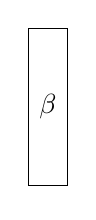
\begin{tikzpicture}[baseline=-0.5ex]
    \draw (0,0) rectangle (.5,2) node[pos=.5] {$\beta$};
\end{tikzpicture}}}
=
\vcenter{\hbox{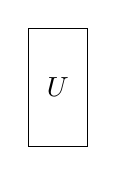
\begin{tikzpicture}[baseline=-0.5ex]
    \draw (0,0) rectangle (.75,1.5) node[pos=.5] {$U$};
\end{tikzpicture}}}
\times
\left(\,
\vcenter{\hbox{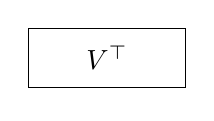
\begin{tikzpicture}[baseline=-0.5ex]
    \draw (0,0) rectangle (2,.75) node[pos=.5] {$V^\top$};
\end{tikzpicture}}}
\times
\vcenter{\hbox{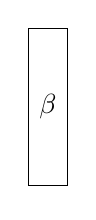
\begin{tikzpicture}[baseline=-0.5ex]
    \draw (0,0) rectangle (.5,2) node[pos=.5] {$\beta$};
\end{tikzpicture}}}
\,\right)
\]
\item Two matrix-vector products of cost $O(LR)$ and $O(L^{|e|}R)$
    \begin{itemize}
    \item Reduced from $O(L^{|e|+1})$
    \end{itemize}
\end{itemize}
\end{frame}

\begin{frame}
\frametitle{Low-rank Hypergraph Marginalization}

Applying the low-rank factorization,

\begin{center}
\begin{algorithm}[H]
%\begin{comment}
\caption{\label{alg:low-rank-update} Low-rank marginalization}
\begin{algorithmic} 
\FOR {$u \leftarrow v_1, v_2$ hyperedge $e$ topologically}
\STATE $\beta_v \gets \alpha_{v_1}\alpha_{v_2}^\top$
    \hfill $\vartriangleright$ $O(L^{|e|})$
\STATE $\gamma \gets V_e^\top\beta_v$
    \hfill $\vartriangleright$ $O(L^{|e|}R)$
\STATE $\alpha_u \stackrel{+}{\gets} U_e\gamma $
    \hfill $\vartriangleright$ $O(LR)$
\ENDFOR
\STATE \textbf{return} $\alpha_S^\top\mathbf{1}$
\end{algorithmic} 
\end{algorithm}
\end{center}

\begin{itemize}
\item Potentially large speedups for marginalization
    \begin{itemize}
    \item HMM from $O(L^2)$ to $O(LR)$
    \item PCFG from $O(L^3)$ to $O(L^2R)$
    \end{itemize}
\end{itemize}


\end{frame}

\begin{frame}
\frametitle{Expressivity of Rank-constrained Models}
\begin{itemize}
\item Rank constraints limit expressivity
\vspace{1em}
\item Only need to constrain bottleneck parameters
    \begin{itemize}
    \item Transition matrix for HMMs
    \item Subset of the transition matrix for PCFGs
    \end{itemize}
\vspace{1em}
\item Is it more expressive than a smaller model?
    \begin{itemize}
    \item An $L$-state HMM with rank $R$ $(< L)$ is more
        expressive than an unconstrained $R$-state HMM
    \end{itemize}
\end{itemize}
\end{frame}

\begin{frame}
\frametitle{Experiments}
\begin{itemize}
\item Language modeling on \textsc{Penn Treebank} \footcite{ptb}
\vspace{1em}
\item Compare size vs speed and accuracy
    \begin{itemize}
    \item Size = 1k to 16k state HMM, 90 to 300 state PCFG
    \item Speed = Sec/Batch
    \item Accuracy = Perplexity (function of likelihood)
    \end{itemize}
\vspace{1em}
\item Unconstrained softmax HMM, PCFG vs low-rank versions %(LHMM, LPCFG)
\vspace{1em}
\item Further experiments in paper
    \begin{itemize}
    \item Polyphonic music modeling with HMMs
    \item Video modeling with HSMMs
    \end{itemize}
\end{itemize}
\end{frame}

\begin{frame}
\frametitle{HMM Accuracy}
\centering
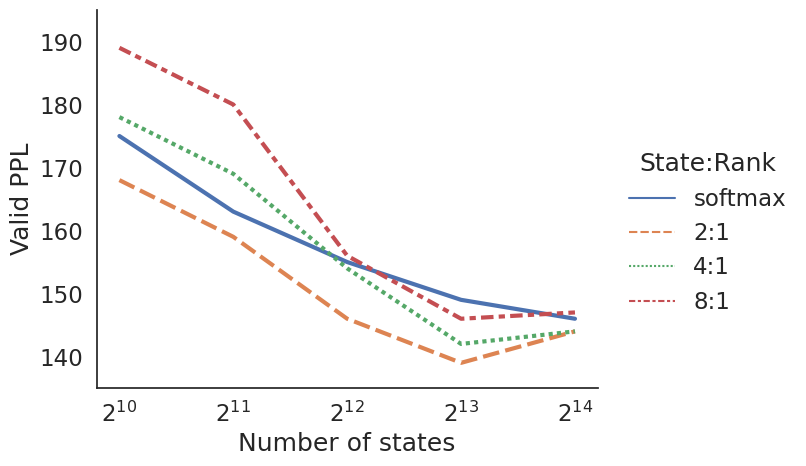
\includegraphics[height=2.5in]{imgs/hmm/lhmm-states-features-dropout.png}
\end{frame}

\begin{frame}
\frametitle{HMM Speed}
\centering
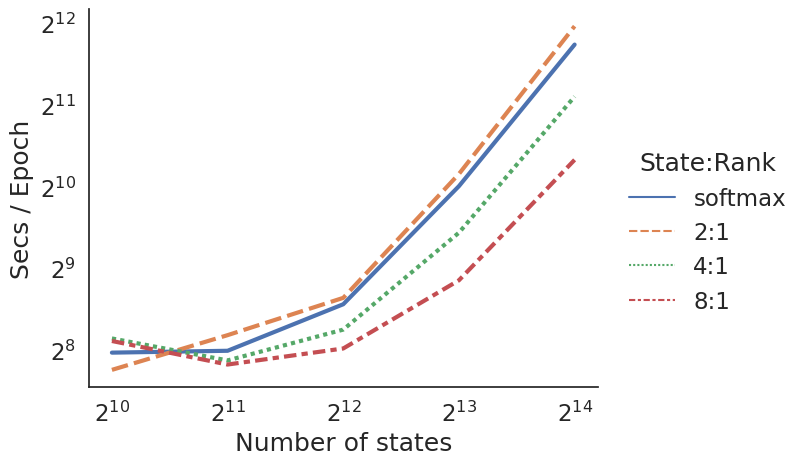
\includegraphics[height=2.5in]{imgs/hmm/lhmm-states-features-speed.png}
\end{frame}

\begin{frame}
\frametitle{HMM Accuracy and Speed}
\centering
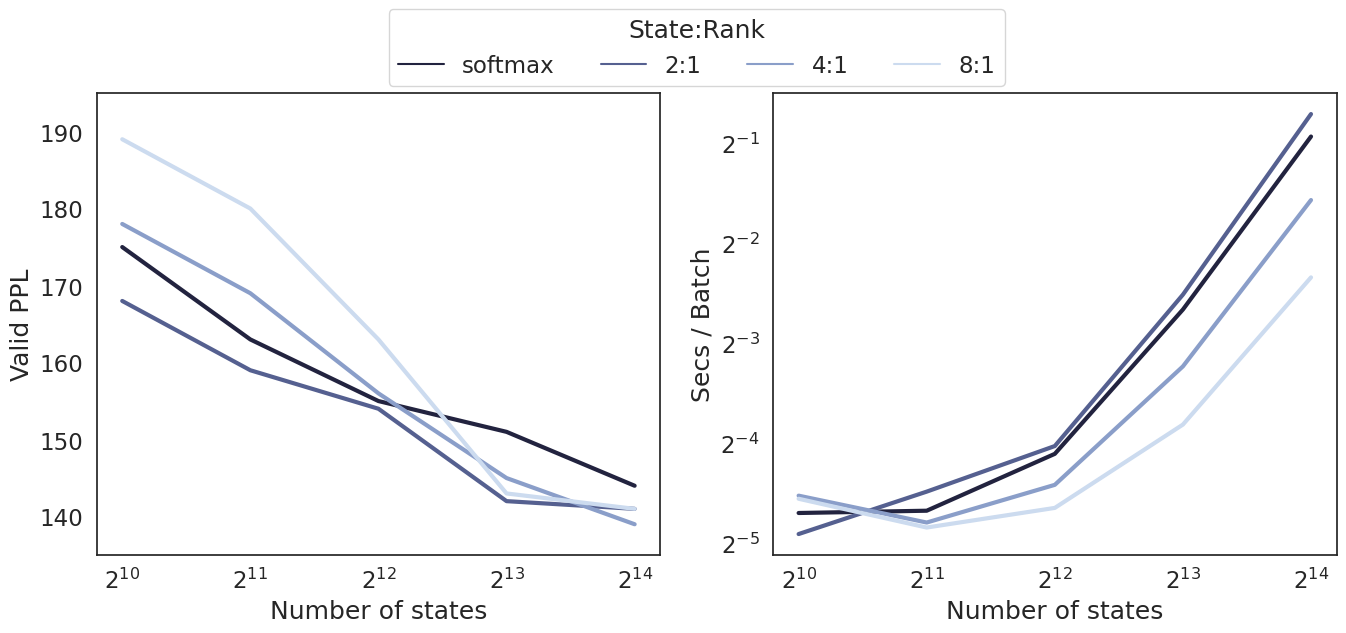
\includegraphics[height=2.1in]{imgs/hmm/lhmm-speed-acc-joint.png}
\end{frame}

\begin{frame}
\frametitle{HMM Speed vs Accuracy Frontier}
\centering
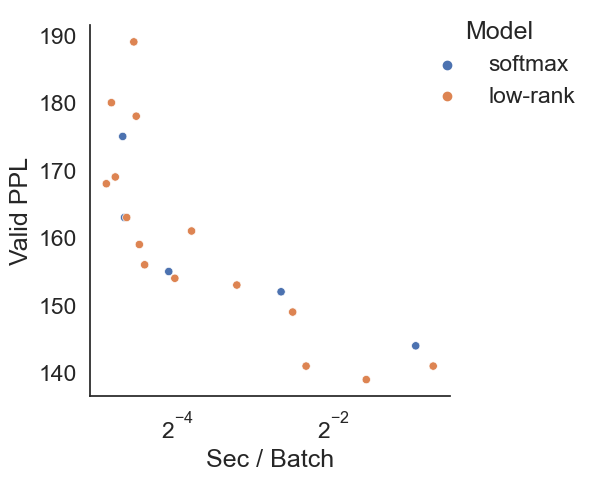
\includegraphics[height=2.5in]{imgs/hmm/lhmm-speed-accuracy.png}
\end{frame}

\begin{frame}
\frametitle{PCFG Speed vs Accuracy Frontier}
\centering
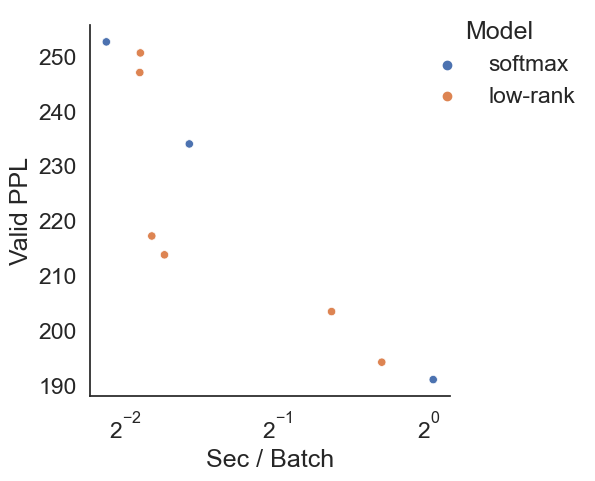
\includegraphics[height=2.5in]{imgs/hmm/pcfg-speed-accuracy.png}
\end{frame}

\begin{frame}
\frametitle{Conclusion}
\begin{itemize}
\item Low-rank factorization speeds up marginalization
    \begin{itemize}
    \item Constrain only bottleneck parameters
    \item Most effective with large models
    \end{itemize}
\vspace{1em}
\item Scaling improves accuracy
    \begin{itemize}
    \item Gap with neural models still large
    \item Scale further with more aggressive constraints
    \item Compose with different representations
    \end{itemize}
\vspace{1em}
\item Please see the paper for more experiments and analysis!
\end{itemize}
\end{frame}


\begin{frame}[allowframebreaks]
\frametitle{Citations}
\printbibliography
\end{frame}



\end{document}
